%%%%%%%%%%%%%%%%%%%%%%%%%%%%%%%%%%%%%%%%%
% Programming/Coding Assignment
% LaTeX Template
%
% This template has been downloaded from:
% http://www.latextemplates.com
%
% Original author:
% Ted Pavlic (http://www.tedpavlic.com)
%
% Note:
% The \lipsum[#] commands throughout this template generate dummy text
% to fill the template out. These commands should all be removed when 
% writing assignment content.
%
% This template uses a Perl script as an example snippet of code, most other
% languages are also usable. Configure them in the "CODE INCLUSION 
% CONFIGURATION" section.
%
%%%%%%%%%%%%%%%%%%%%%%%%%%%%%%%%%%%%%%%%%

%----------------------------------------------------------------------------------------
%	PACKAGES AND OTHER DOCUMENT CONFIGURATIONS
%----------------------------------------------------------------------------------------

\documentclass{article}

\usepackage{fancyhdr} % Required for custom headers
\usepackage{lastpage} % Required to determine the last page for the footer
\usepackage{extramarks} % Required for headers and footers
\usepackage[usenames,dvipsnames]{color} % Required for custom colors
\usepackage{graphicx} % Required to insert images
\usepackage{listings} % Required for insertion of code
\usepackage{courier} % Required for the courier font
\usepackage{lipsum} % Used for inserting dummy 'Lorem ipsum' text into the template
\usepackage{setspace}
\usepackage{color}
\usepackage{comment}
\usepackage{caption}

\usepackage{hyperref}
\usepackage{natbib}
\usepackage{underscore}
\usepackage{subfigure}
\usepackage{fixltx2e}

\hypersetup{
    colorlinks=true,
    linkcolor=blue,
    filecolor=magenta,      
    urlcolor=cyan,
    breaklinks=true
}

%\usepackage[]{algorithm2e}
\usepackage{pdfpages}




%For python inclusion (http://widerin.org/blog/syntax-highlighting-for-python-scripts-in-latex-documents)
\definecolor{Code}{rgb}{0,0,0}
\definecolor{Decorators}{rgb}{0.5,0.5,0.5}
\definecolor{Numbers}{rgb}{0.5,0,0}
\definecolor{MatchingBrackets}{rgb}{0.25,0.5,0.5}
\definecolor{Keywords}{rgb}{0,0,1}
\definecolor{self}{rgb}{0,0,0}
\definecolor{Strings}{rgb}{0,0.63,0}
\definecolor{Comments}{rgb}{0,0.63,1}
\definecolor{Backquotes}{rgb}{0,0,0}
\definecolor{Classname}{rgb}{0,0,0}
\definecolor{FunctionName}{rgb}{0,0,0}
\definecolor{Operators}{rgb}{0,0,0}
\definecolor{Background}{rgb}{0.98,0.98,0.98}

% Margins
\topmargin=-0.45in
\evensidemargin=0in
\oddsidemargin=0in
\textwidth=6.5in
\textheight=9.0in
\headsep=0.25in

\linespread{1.1} % Line spacing

% Set up the header and footer
\pagestyle{fancy}
\lhead{\hmwkAuthorName} % Top left header
%\chead{\hmwkClass\ (\hmwkClassInstructor\ \hmwkClassTime): \hmwkTitle} % Top center head
\chead{\hmwkClass\ (\hmwkClassInstructor): \hmwkTitle} % Top center head
\rhead{\firstxmark} % Top right header
\lfoot{\lastxmark} % Bottom left footer
\cfoot{} % Bottom center footer
\rfoot{Page\ \thepage\ of\ \protect\pageref{LastPage}} % Bottom right footer
\renewcommand\headrulewidth{0.4pt} % Size of the header rule
\renewcommand\footrulewidth{0.4pt} % Size of the footer rule

\setlength\parindent{0pt} % Removes all indentation from paragraphs

%----------------------------------------------------------------------------------------
%	CODE INCLUSION CONFIGURATION
%----------------------------------------------------------------------------------------

\definecolor{MyDarkGreen}{rgb}{0.0,0.4,0.0} % This is the color used for comments
\lstloadlanguages{Perl} % Load Perl syntax for listings, for a list of other languages supported see: ftp://ftp.tex.ac.uk/tex-archive/macros/latex/contrib/listings/listings.pdf
\lstset{language=Perl, % Use Perl in this example
        frame=single, % Single frame around code
        basicstyle=\small\ttfamily, % Use small true type font
        keywordstyle=[1]\color{Blue}\bf, % Perl functions bold and blue
        keywordstyle=[2]\color{Purple}, % Perl function arguments purple
        keywordstyle=[3]\color{Blue}\underbar, % Custom functions underlined and blue
        identifierstyle=, % Nothing special about identifiers                                         
        commentstyle=\usefont{T1}{pcr}{m}{sl}\color{MyDarkGreen}\small, % Comments small dark green courier font
        stringstyle=\color{Purple}, % Strings are purple
        showstringspaces=false, % Don't put marks in string spaces
        tabsize=5, % 5 spaces per tab
        %
        % Put standard Perl functions not included in the default language here
        morekeywords={rand},
        %
        % Put Perl function parameters here
        morekeywords=[2]{on, off, interp},
        %
        % Put user defined functions here
        morekeywords=[3]{test},
       	%
        morecomment=[l][\color{Blue}]{...}, % Line continuation (...) like blue comment
        numbers=left, % Line numbers on left
        firstnumber=1, % Line numbers start with line 1
        numberstyle=\tiny\color{Blue}, % Line numbers are blue and small
        stepnumber=5 % Line numbers go in steps of 5
}

% Creates a new command to include a perl script, the first parameter is the filename of the script (without .pl), the second parameter is the caption
\newcommand{\perlscript}[2]{
\begin{itemize}
\item[]\lstinputlisting[caption=#2,label=#1]{#1.pl}
\end{itemize}
}


%----------------------------------------------------------------------------------------
%	DOCUMENT STRUCTURE COMMANDS
%	Skip this unless you know what you're doing
%----------------------------------------------------------------------------------------

% Header and footer for when a page split occurs within a problem environment
\newcommand{\enterProblemHeader}[1]{
\nobreak\extramarks{#1}{#1 continued on next page\ldots}\nobreak
\nobreak\extramarks{#1 (continued)}{#1 continued on next page\ldots}\nobreak
}

% Header and footer for when a page split occurs between problem environments
\newcommand{\exitProblemHeader}[1]{
\nobreak\extramarks{#1 (continued)}{#1 continued on next page\ldots}\nobreak
\nobreak\extramarks{#1}{}\nobreak
}

\setcounter{secnumdepth}{0} % Removes default section numbers
\newcounter{homeworkProblemCounter} % Creates a counter to keep track of the number of problems

\newcommand{\homeworkProblemName}{}
\newenvironment{homeworkProblem}[1][Problem \arabic{homeworkProblemCounter}]{ % Makes a new environment called homeworkProblem which takes 1 argument (custom name) but the default is "Problem #"
\stepcounter{homeworkProblemCounter} % Increase counter for number of problems
\renewcommand{\homeworkProblemName}{#1} % Assign \homeworkProblemName the name of the problem
\section{\homeworkProblemName} % Make a section in the document with the custom problem count
\enterProblemHeader{\homeworkProblemName} % Header and footer within the environment
}{
\exitProblemHeader{\homeworkProblemName} % Header and footer after the environment
}

\newcommand{\problemAnswer}[1]{ % Defines the problem answer command with the content as the only argument
\noindent\framebox[\columnwidth][c]{\begin{minipage}{0.98\columnwidth}#1\end{minipage}} % Makes the box around the problem answer and puts the content inside
}

\newcommand{\homeworkSectionName}{}
\newenvironment{homeworkSection}[1]{ % New environment for sections within homework problems, takes 1 argument - the name of the section
\renewcommand{\homeworkSectionName}{#1} % Assign \homeworkSectionName to the name of the section from the environment argument
\subsection{\homeworkSectionName} % Make a subsection with the custom name of the subsection
\enterProblemHeader{\homeworkProblemName\ [\homeworkSectionName]} % Header and footer within the environment
}{
\enterProblemHeader{\homeworkProblemName} % Header and footer after the environment
}

%----------------------------------------------------------------------------------------
%	NAME AND CLASS SECTION
%----------------------------------------------------------------------------------------
%#MOD
\newcommand{\hmwkTitle}{Assignment\ \#2 } % Assignment title
%\newcommand{\hmwkDueDate}{Monday,\ January\ 1,\ 2012} % Due date
\newcommand{\hmwkClass}{Introduction to Digital Libraries} % Course/class
%\newcommand{\hmwkClassTime}{10:30am} % Class/lecture time
\newcommand{\hmwkClassInstructor}{Dr. Nelson} % Teacher/lecturer
\newcommand{\hmwkAuthorName}{Alexander Nwala} % Your name

%----------------------------------------------------------------------------------------
%	TITLE PAGE
%----------------------------------------------------------------------------------------

\title{
\vspace{2in}
\textmd{\textbf{\hmwkClass:\ \hmwkTitle}}\\
%\normalsize\vspace{0.1in}\small{Due\ on\ \hmwkDueDate}\\
%\vspace{0.1in}\large{\textit{\hmwkClassInstructor\ \hmwkClassTime}}
\vspace{0.1in}\large{\textit{\hmwkClassInstructor}}
\vspace{3in}
}

\author{\textbf{\hmwkAuthorName}}
%#MOD
\date{Thursday, March 5, 2015} % Insert date here if you want it to appear below your name

%----------------------------------------------------------------------------------------

\begin{document}

\maketitle



%----------------------------------------------------------------------------------------
%	TABLE OF CONTENTS
%----------------------------------------------------------------------------------------

%\setcounter{tocdepth}{1} % Uncomment this line if you don't want subsections listed in the ToC

\newpage
\tableofcontents
\newpage

%----------------------------------------------------------------------------------------
%	PROBLEM 1
%----------------------------------------------------------------------------------------

% To have just one problem per page, simply put a \clearpage after each problem

\begin{homeworkProblem}

Choose 100 URIs from A1
Generate WARC files of those URIs using:
\begin{enumerate}
\item wget
\item WARCreate
\item Heritrix (stand-alone or via WAIL)
\item webrecorder.io
\end{enumerate}
Describe the resulting WARC files: quantitatively compare \& contrast the results of the WARC files of the same URI as generated by different tools.
Choose interesting examples
Demonstrate playback of 2-3 WARCs in the (Wayback Machine (via WAIL or stand-alone) or pywb) and (webrecorder.io)
\url{https://github.com/iipc/openwayback},  
\url{https://github.com/ikreymer/pywb}


%\problemAnswer
%{
    \begin{verbatim}\end{verbatim}
    \textbf{SOLUTION}\\


    The solution for this problem is outlined by the following steps:
    \begin{enumerate}

    \item \textbf{Generating WARC files with wget:} wget \cite{wget} provides a functionality to create single WARC files from multiple URIs as outlined below.

    \begin{verbatim}
        $ wget --warc-file=outputFileName -p -l 1 URI0 URI1 ... URIN
    \end{verbatim}

    Using this functionality, Listing 1. outlines the procedure of generating 2 WARC files - one file for the first 50 URIs, and the second - for the last 50 URIs. Only one level of crawl (-l 1 option) was used to generate the WARC files. The outcome of using wget was 2 WARC files of size 3.7MB and 6.7MB.



    \lstinputlisting[breaklines=true, caption=Generate WARC file]{wgetGenWarcFileSnippet.py}

    \item \textbf{Generating WARC files with WARCreate:} WARCreate \cite{WARCreate} provides a means to preserve a single page at a time. Consequently, in order to generate WARC files, I visited each URI from the list of 100 and clicked WARCreate's ``Generate WARC'' button in order to download the WARC files for the respective URIs. 60 WARC files were created from the set of 100. The outcome of using WARCreate was 60 WARC files of total size 998.8MB.
    \\ \\
    Given that WARCreate does not consolidate multiple WARC files from multiple URIs, the following command was used in order to generate a single WARC file from the set:
    \begin{verbatim}
        cat *.warc > *.outputFileName.warc
    \end{verbatim}



    \item \textbf{Generating WARC files with Heritrix via WAIL:} WAIL (Windows version) \cite{WAIL} was used to crawl the set of URIs to generate a single WARC file. The outcome of using WAIL was 1 WARC file of size 120.8MB. The following outlines the procedure for configuring WAIL to generate the WARC file:

    \begin{verbatim}
        1. From windows command prompt, cmd.exe
            cd C:\WAIL
        2. From C:\WAIL
            python WAIL.py
        3. From WAIL GUI
            Advanced > setup-one crawl > click top empty textbox > 
            add URI > write - heritrix config
        4. From C:\WAIL\jobs\
            From crawler-bean.cxml
                From section "URLS HERE"
                    Add URIs to crawl
                From section "CRAWLLIMITENFORCER"
                    Set the following properties:
                    <property name="maxBytesDownload" value="100000000" /> 
                    <property name="maxDocumentsDownload" value="10000" />
                    <property name="maxTimeSeconds" value="10800" />
        5. save crawler-bean.cxml
        6. From WAIL GUI
            From Advanced Tab
                Click Launch crawl
                Click View in Heritrix browser
        7. From browser
            Click job
                Click launch
    \end{verbatim}


    \item \textbf{Generating WARC files with webrecorder.io:} webrecorder.io \cite{webrecorder}
    provides a means of archiving URIs and downloading the archived URIs into a single WARC file. Using the webrecorder.io service online, I recorded the first URI, then continued to record others by adding new URIs and clicking on the reload button. Finally I downloaded the resultant WARC file. The outcome of using webrecorder.io was 1 WARC file of size 119.8MB
   

    
    \end{enumerate}

    Consider Table 1. for comparison of the WARC files as generated by the different methods.
   
    \begin{table}
    \caption{Comparison Of The Different Methods} % title of Table
    \centering % used for centering table
    \begin{tabular}{c | c | c | c | c | c} % centered columns (4 columns)
    \hline\hline %inserts double horizontal lines
    Method & Count of WARCs & Concurrency & Ease of Use & Recommended User & Crawl scope  \\ [0.5ex] % inserts table 
    %heading
    \hline \hline% inserts single horizontal line
    wget   &   Multiple    &   Yes & Medium & Advanced Archivist & Large \\ \hline
    WARCreate   &   Single    &  No & Easy & Beginner Archivist & Small\\ \hline
    WAIL   &   Multiple    &   Yes & Hard & Advanced Archivist & Large \\ \hline
    webrecorder.io & Multiple & No & Easy & Beginner Archivist & Small \\ [1ex] 
    \hline %inserts single line
    \end{tabular}
    \label{table:nonlin} % is used to refer this table in the text
    \end{table}

    \begin{table}
    \caption{Comparison Of The WARC Files} % title of Table
    \centering % used for centering table
    \begin{tabular}{c | c | c | c } % centered columns (4 columns)
    \hline\hline %inserts double horizontal lines
    Method & Size (MB) & URIs Count & Page Count \\ [0.5ex] % inserts table 
    %heading
    \hline \hline% inserts single horizontal line
    wget   &   2.57    &   103 & 14  \\ \hline
    WARCreate   &   8.99    &  74 & 1  \\ \hline
    WAIL   &   11.02    &   158 & 31  \\ \hline
    webrecorder.io & 13.57 & 68 & 3  \\ [1ex] 
    \hline %inserts single line
    \end{tabular}
    \label{table:nonlin} % is used to refer this table in the text
    \end{table}

    Consider the following comparison based on crawl control:
    
    \begin{enumerate}
        \item \textbf{wget:} wget provides a means to set the crawl level.
        \item \textbf{WARCreate:} WARCreate does not expose any means to set the crawl level.
        \item \textbf{WAIL:} WAIL exposes the Heritrix setting to control the crawl by setting limits on the maximum size of crawl (maxBytesDownload), the maximum number of files to download (maxDocumentsDownload), the maximum time to be spent crawling (maxTimeSeconds). 
        \item \textbf{webrecorder.io:} webrecorder.io enables the user to interactively explore pages to be archived.
    \end{enumerate}
   
 
    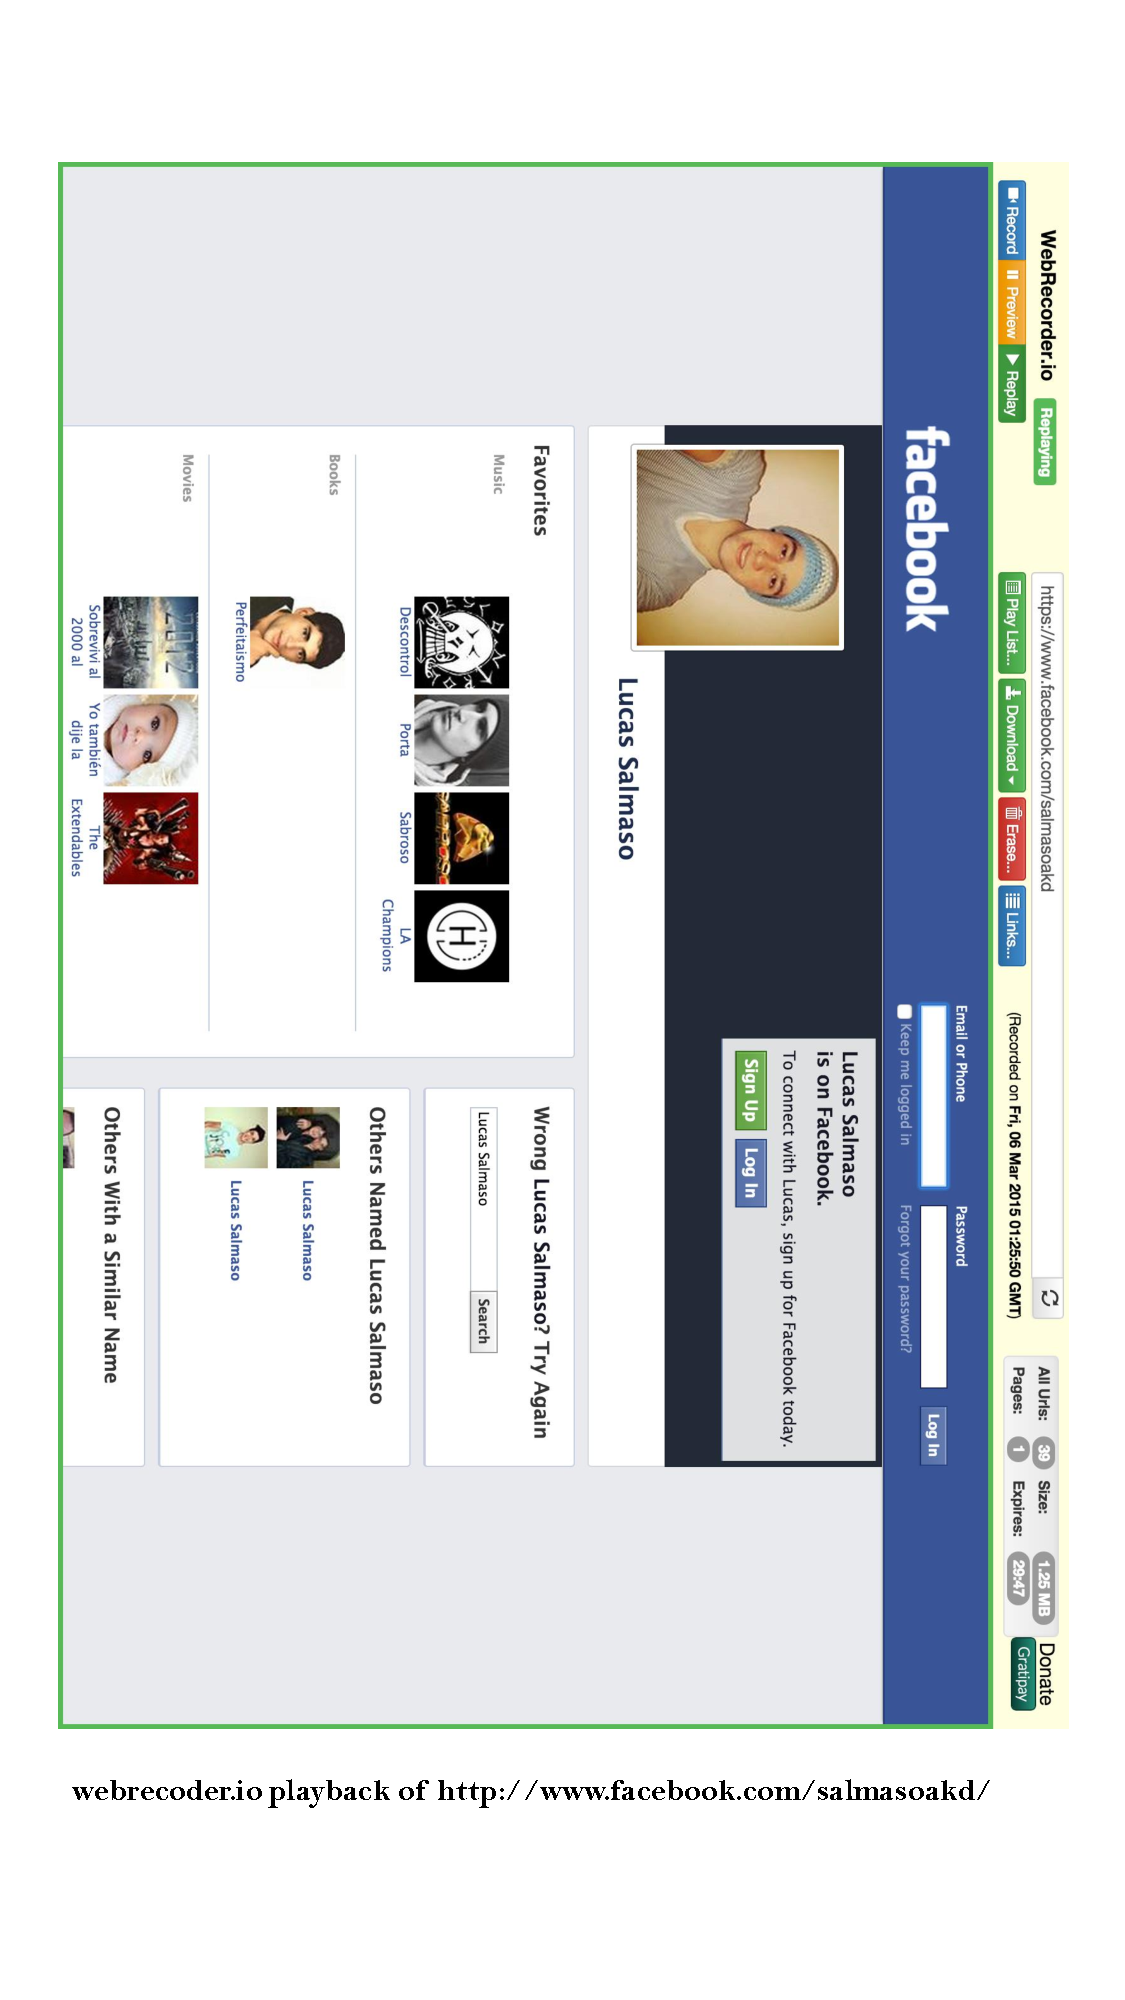
\includepdf[scale=1.0,pages=1]{playBack1.pdf}
    \includepdf[scale=1.0,pages=2]{playBack1.pdf}



  



%}

\end{homeworkProblem}

%----------------------------------------------------------------------------------------
%   PROBLEM 2
%----------------------------------------------------------------------------------------

\begin{homeworkProblem}

Ingest the 100 URIs from their resulting WARC files into a SOLR instance
see the code + tutorial at: \url{https://github.com/ukwa/webarchive-discovery}
\\ \\ Demonstrate several functioning queries on the files (a full front-end is not required)
describe the configuration choices you made in setting up SOLR and processing the documents


%\problemAnswer
%{
    \begin{verbatim}\end{verbatim}
    \textbf{SOLUTION}\\


    The solution for this problem is outlined by the following steps:\\ \\
   

   \textbf{SOLR Configurations:} Consider the following setting:


    \begin{verbatim}
From solrconfig.xml: Keep the default cache size of 512 

From schema.xml: Change the restrictive "AND" default solrQueryParser 
to "OR," in order to increase recall at the expense of Precision.
 
From stopwords.txt: Populate with list from http://www.ranks.nl/stopwords, 
in order to filter out stopwords
    \end{verbatim}

   \textbf{Query 1: } Consider the excerpts of output for query - ``food''
   \begin{verbatim}
    "source_file_s": "MAT-2.warc@77683046",
    "url": "https://foursquare.com/",
    ...
   "content": [
          "Norfolk | Food, Nightlife, EntertainmentFoursquare
          Log InSign UpHere are some popular tips in Norfolk. 
          Select a taste to see more:Beer gardensHealthy foodCocktailsGood 
          for workingMexican foodTrendy placesPhilly 
          cheesesteaksBagelsSeafoodFoursquare
        ],
   \end{verbatim}

   \textbf{Query 2: } Consider the excerpts of output for query - ``healthcare''
   \begin{verbatim}
    "content": [
          "You Can't Understand ISIS If You Don't Know the History 
          of Wahhabism in Saudi Arabia | Alastair... - 
          Linkis.comClose panel
          http://www.huffingtonpost.com/alastair-crooke/isis-
          wahhabism-saudi-arabia_b_5717157.html?utm_hp_ref=tw4 views• tweets
          You Can't Understand #ISIS
   \end{verbatim}


   \begin{verbatim}
The files q1.json and q2.json contain the complete data for "food" 
and "healthcare" queries respectively
   \end{verbatim}

   \begin{figure}

    \caption{Snapshot of SOLR local server}
    \subfigure[Output for Query Food]{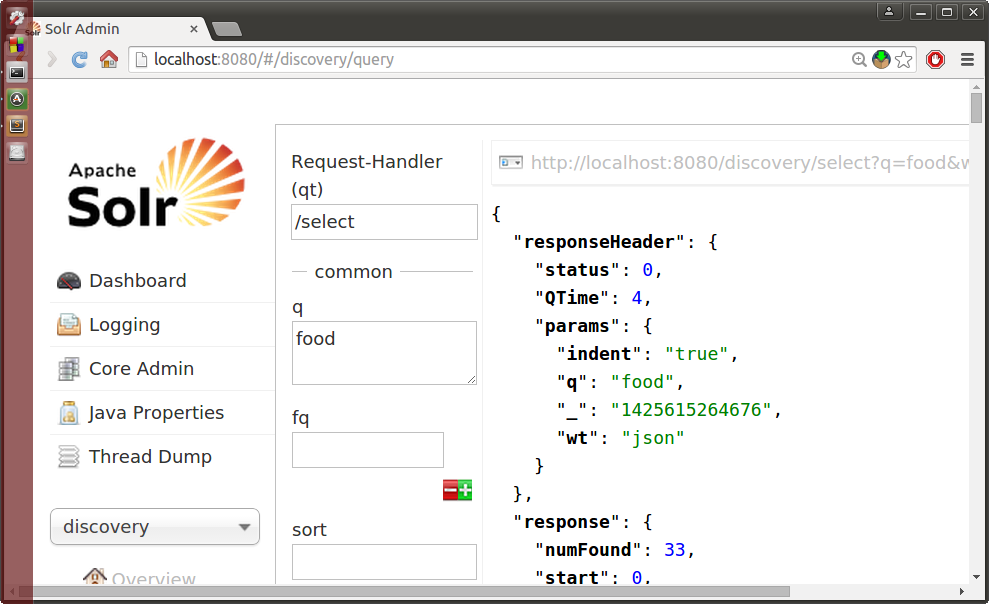
\includegraphics[width=\textwidth]{sl1.png}}
    \subfigure[Output for Query Healthcare]{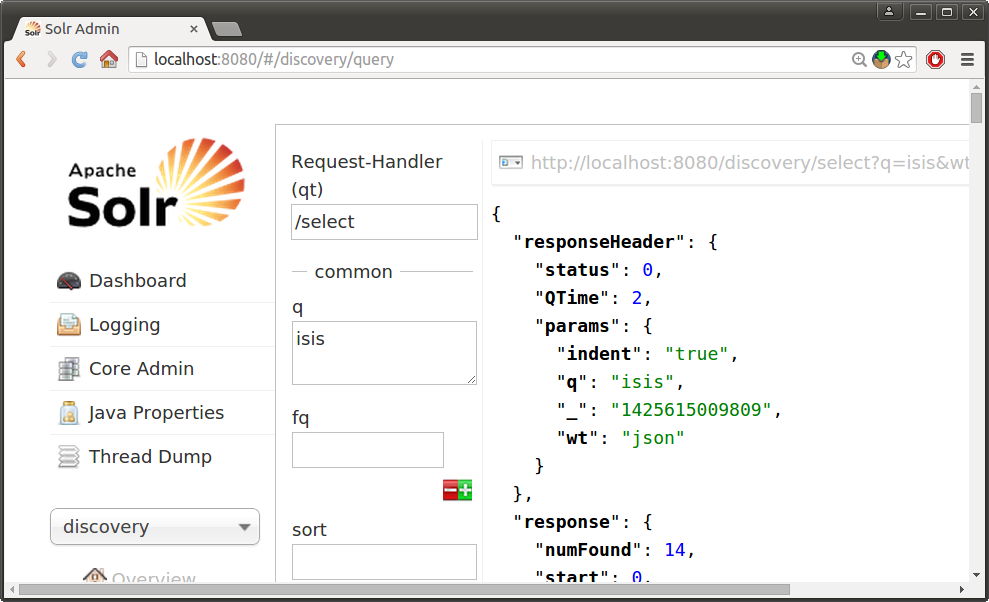
\includegraphics[width=\textwidth]{sl2.png}}

   \end{figure}
    


   

    

    

    
   

%}

\end{homeworkProblem}
\bibliographystyle{plain}
\bibliography{A2bibFile}

\end{document}

\begin{comment}
\begin{figure}

    \caption{Multiple Iterations Of The Girvin-Newman Algorithm}
    \subfigure[Iteration: 20, Clusters: 4]{\includegraphics[width=.50\textwidth]{../graphs/sn-20-4.pdf}}
    \subfigure[Iteration: 21, Clusters: 4]{\includegraphics[width=.50\textwidth]{../graphs/sn-21-4.pdf}}
    \subfigure[Iteration: 22, Clusters: 4]{\includegraphics[width=.50\textwidth]{../graphs/sn-22-4.pdf}}
    \subfigure[Iteration: 23, Clusters: 4]{\includegraphics[width=.50\textwidth]{../graphs/sn-23-4.pdf}}

\end{figure}
\end{comment}